\section{Task and setup}\label{sec:task}
\begin{figure}[tb]
\centering
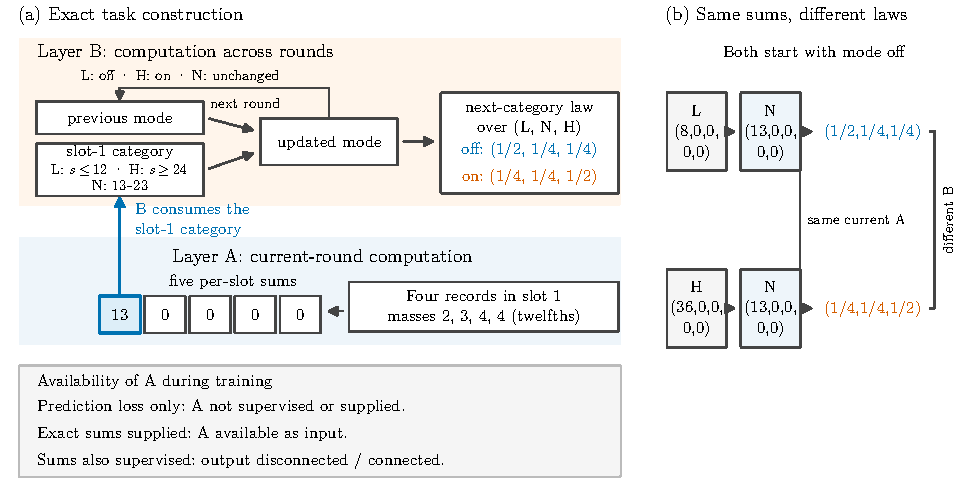
\includegraphics[width=\textwidth]{figures/fig1.pdf}
\caption{\csname captionfig1\endcsname}\label{fig:fig1}
\end{figure}

\begin{figure}[tb]
\centering
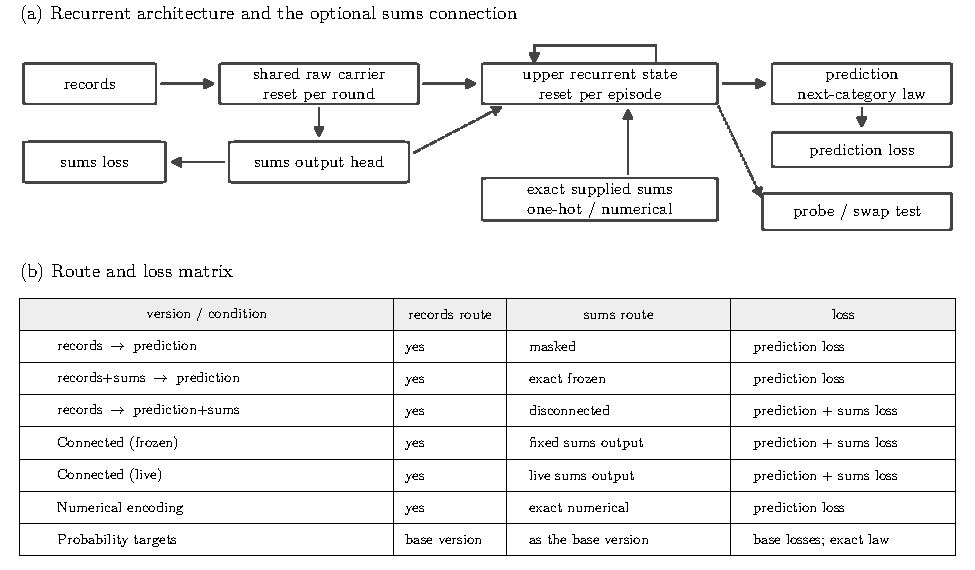
\includegraphics[width=\textwidth]{figures/fig2.pdf}
\caption{\csname captionfig2\endcsname}\label{fig:fig2}
\end{figure}


In the records game, the quantities a network might compute, the hidden
variable and the correct next-step probabilities are known exactly for every
input, and all boards can be enumerated (\cref{fig:fig1}).

\subsection{The game}\label{sec:game}

\paragraph{Boards and sums.} A \emph{record} places one mass in one of five
\emph{slots}. The six masses are $1/6$, $1/4$, $1/3$, $1/2$, $2/3$ and $3/4$,
written below in integer twelfths (2, 3, 4, 6, 8, 9). A \emph{board} is an
ordered sequence of four records. Its \emph{sums} are the five per-slot
totals, each one of the 36 attainable values $0$ and $2$--$36$ twelfths.
Computing the sums defines layer~A. The $30^4 = 810{,}000$ ordered placements
yield 24,435 distinct \emph{completed sum boards}; many record sequences
realize the same completed sum board, and we call one such realization a
\emph{rendering}.

\paragraph{Category, mode and law.} Only slot~1 matters for prediction. Its
sum gives the board's \emph{slot-1 category}: \Lcat{} when the sum is at most
12 twelfths, \Hcat{} when it is at least 24, and \Ncat{} otherwise (13--23).
The task keeps a binary \emph{mode}, which starts off. An \Hcat{} board
switches it on, an \Lcat{} board switches it off, and an \Ncat{} board leaves
it unchanged. The next board's category is drawn from the \emph{law}
$(\tfrac12, \tfrac14, \tfrac14)$ over $(\Lcat, \Ncat, \Hcat)$ when the mode
is off and $(\tfrac14, \tfrac14, \tfrac12)$ when it is on. Given the
category, the next board is a uniformly chosen completed sum board of that
category, rendered as a legal placement of records. At every round the
network sees the current board's records and outputs a \emph{prediction}: a
probability vector over the next board's category. Predicting the law is the
upper task layer~B. In the \emph{equal-law control} both modes use
$(\tfrac38, \tfrac14, \tfrac38)$, so the mode is irrelevant; it checks that
the measurements do not report mode use where none is possible.

\paragraph{Boards near the cutoffs.} 22,491 completed sum boards are
\Lcat{}, 1,835 are \Ncat{} and 109 are \Hcat{}. The \emph{cutoff band}
(slot-1 sums 11--13 and 23--25; 930 boards) is 2.5\% of the \Lcat{} boards,
16.9\% of the \Ncat{} boards and 45.9\% of the \Hcat{} boards. Under uniform
sampling within a category, these shares are also the training probability
of a band board; the rarity conditions of r11 and r12 change them.

\subsection{Two task layers}\label{sec:strict}

Layer A maps each round's records to its five sums. Layer B operates over
sequences of these completed sum boards: the slot-1 category updates the
preceding mode, and the updated mode determines the next-category law
(\cref{fig:fig1}a). The exact update needs only two things, the current
board's slot-1 category and the previous mode. A network that predicts
reliably must therefore combine information about the current board's
category with information from earlier boards; it need not do so through the
exact sums.

Six Birds Theory gives this relationship a precise meaning. A description B
\emph{strictly extends} a description A when B draws distinctions that no
function of A can draw. The theory uses this as its certificate of novelty:
a new level of description adds predicates that are not definable from the
old one, rather than computing further within it
\citep[\S1.1]{tsiokos2026foundations}. Formally, B does not factor through A,
which holds exactly when some pair of cases has equal A and different B
(\citealp[Theorem~12]{tsiokos2026foundationsiii};
\citealp[\S3.5]{tsiokos2026strict}); this non-factorization is the only
condition we use. Under the original law, B (the next-category law) strictly
extends the current A description (the five sums): no function of the
current sums gives the correct law for every history. Two histories ending on
the same neutral board have identical sums but can retain different modes
and require different laws (\cref{fig:fig1}b). B is determined by the
sequence of A objects and the initial mode, not by the current A object
alone. Neither containment nor recovery of A from B is required. The
equal-law control removes this distinction.

These are the task's layers. Whether training realizes their decomposition
internally is the empirical question.

\subsection{Network, versions and training}\label{sec:versions}

\paragraph{Network.} For the original task all networks share one
architecture (\cref{fig:fig2}); in r10 the upper state also receives the
public query. Within a round, a one-layer GRU of width 16 reads the four
records and produces the \emph{raw carrier}, which is reset at every round.
Across rounds, an upper GRU cell of width 32 receives the raw carrier and,
where a version provides them, the five sums as one-hot vectors; a linear
head on the upper state gives the prediction. Supplied sums come from a
separately trained sums network that is exact on all 1,555 local histories
(every ordered sequence of up to four masses in one slot) and is kept
frozen. Details are in \cref{app:training}.

\paragraph{Versions.} Each version name states the input, an arrow, and what
the loss is computed on. In \textbf{records $\to$ prediction} the input is
the records and the loss is on the prediction only. In \textbf{records+sums
$\to$ prediction} the input also includes the exact one-hot sums. In
\textbf{records $\to$ prediction+sums} the input is the records and the loss
is on the prediction plus a \emph{sums output}, a linear head on the raw
carrier trained to give the five sums and not fed to the prediction.
r8 trained the first two versions and a third, \textbf{records+sums $\to$
prediction (sums route only)}, whose upper state receives only the exact
sums; records $\to$ prediction+sums first appears in r10. The versions vary the supervision of A and
its availability to B: no explicit sums supervision, exact supplied sums, or
supervised sums outputs disconnected from or connected to prediction.
Further variants change one factor. \textbf{Connected (frozen)} and \textbf{Connected (live)}
feed the sums output of a trained records $\to$ prediction+sums network into
the prediction, from a fixed copy or from the sums output being trained.
\textbf{Numerical encoding} gives the exact sums as $(s/36,\,1-s/36)$ per
slot instead of one-hot. \textbf{Probability targets} train against the
exact law instead of one sampled next category. The \textbf{erosion
continuation} starts from an exact sums network that is no longer frozen and
updates either the prediction loss only or the prediction plus sums loss.

\paragraph{Training.} Full training runs use three seeds (0, 1, 2), a fixed
20,000 updates, AdamW (learning rate 0.003, weight decay 0.01, batch 256),
float32 and freshly drawn episodes; no checkpoint is selected by accuracy.
From r12 on, each batch also contains \emph{history coverage}: constructed
prefixes of an \Lcat{} or \Hcat{} board followed by up to eight \Ncat{}
boards. The r13 erosion replays instead run for 200 updates and compare
three optimizers for the sums network (AdamW, AdamW with a tenfold smaller
learning rate, and SGD matched to the norm of AdamW's first gradient-only displacement) with a control that
blocks the prediction gradient to the sums network while weight decay
continues. r9 trains nothing. Details are in \cref{app:training}.

\subsection{Study history and comparisons}\label{sec:history}

The evidence comes from six studies, r8--r13, each registered with its
endpoints and criteria before it ran. r8 trained the three r8 networks under
both laws. r9 diagnosed the saved r8 networks. r10 retains A but changes B to the
\emph{all-slots task}, testing readability and use of all five sums: there
each slot remembers its last nonzero sum (initially zero) and the law over
the next board's total sum modulo three depends on the remembered value of a
publicly queried slot, not its current sum (36 distinct laws). r11 varied board
rarity near the cutoffs, the amount of sums supervision, and the erosion
continuation. r12 added history coverage. r13 ran four mechanism experiments:
target noise, access, encoding and erosion. Follow-ups, corrected audits and
supplementary analyses are labeled in \cref{app:history}; the campaign was
not one confirmatory study.

A comparison is \emph{matched} when the code, data streams, initialization,
number of updates and evaluation panels are identical and only the stated
factor differs. All other comparisons are \emph{historical}. Comparisons
between r11 and r12 change the curriculum and the loss weighting at once;
comparisons between r10 and the other studies change the task. The r13
access and encoding experiments share one reference condition, the exact
one-hot supplied sums, which we count once.
